The three lower bounds use one and the same original tile $F$.
Its actual bottom chord has length
$b_F\ge2\mu-\Sigma$, and it contains the lower axial tip $D_C$.
Its diameter gives $b_F\le\sqrt2$, hence
$\Sigma\ge2\mu-\sqrt2>2-\sqrt2$.
The three-axis unit-square inequality applied to this chord and tip gives
$b_F+(\mu-d)^2\le2$, so
$\Sigma\ge2\mu-2+(\mu-d)^2>(1-d)^2$.
For the last bound, the triangle with the two bottom-gap endpoints and $D_C$
has area at most $1/2$:
\[
 (2\mu-\Sigma)(\mu-d)\le1.
\]
Since $d<1<\mu$, it follows that
$\Sigma\ge2\mu-1/(\mu-d)>2-1/(1-d)$.
The chord endpoints and the axial tip cannot be supplied by different
placements of $F$.

\begin{figure}[htbp]\centering
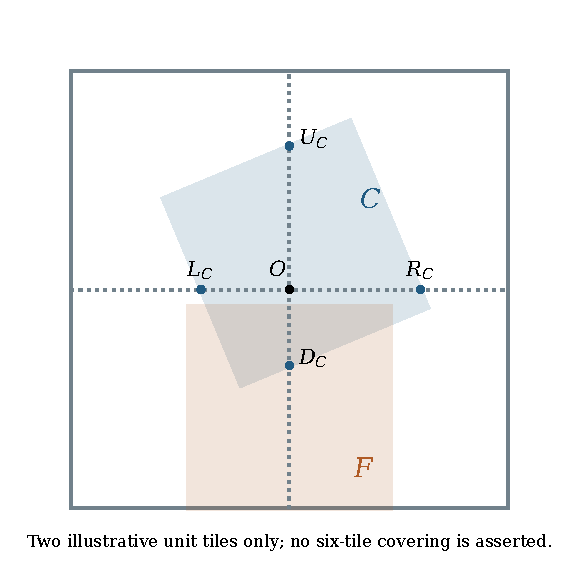
\includegraphics[width=.72\textwidth]{figures/07_final_axes.pdf}
\caption{Actual axial tips of one illustrative rotated unit tile, and an
illustrative unit tile below $H_0$. Only two tiles are shown; no six-tile
covering is asserted. The argument requires the same $F$ to contain the
bottom-gap endpoints and $D_C$.}
\label{fig:final-axes}\end{figure}

